
\documentclass[10pt]{article}
\linespread{1.25}

%%Make Parenthesis scale to fit whats inside
\newcommand{\parry}[1]{\left( #1 \right)}

%% Language and font encodings
\usepackage[english]{babel}
\usepackage[utf8x]{inputenc}
\usepackage[T1]{fontenc}
\usepackage{subcaption}
\usepackage[section]{placeins}

%% Sets page size and margins
\usepackage[a4paper,top=3cm,bottom=2cm,left=3cm,right=3cm,marginparwidth=1.75cm]{geometry}

%% No indents
\setlength\parindent{0pt}

%% Useful packages
\usepackage{amsmath}
\usepackage{amssymb}
\usepackage{amsfonts}
\usepackage{mathtools}
\usepackage{graphicx}
\usepackage{xcolor}
\usepackage[colorinlistoftodos]{todonotes}
\usepackage[colorlinks=true, allcolors=blue]{hyperref}
\usepackage{enumerate}
\usepackage{enumitem}
\usepackage[framed,autolinebreaks,useliterate]{mcode} %% MATLAB code
\usepackage{siunitx}
\usepackage{float}
\usepackage{scrextend}
\usepackage[final]{pdfpages}

%%Header & Footer
\usepackage[myheadings]{fullpage}
\usepackage{fancyhdr}
\usepackage{lastpage}
\usepackage{graphicx, wrapfig, subcaption, setspace, booktabs}

%% Define \therefore command
\def\therefore{\boldsymbol{\text{ }
\leavevmode
\lower0.4ex\hbox{$\cdot$}
\kern-.5em\raise0.7ex\hbox{$\cdot$}
\kern-0.55em\lower0.4ex\hbox{$\cdot$}
\thinspace\text{ }}}
\renewcommand{\vec}[1]{\boldsymbol{#1}}

%% Units
\DeclareSIUnit\year{yr}
\DeclareSIUnit\dollar{\$}
\DeclareSIUnit\celcius{C^{\circ}}
\DeclareSIUnit\mole{mole}
\def\conclusion{\quad \Rightarrow \quad}

\begin{document}


%----------------------------------------------------------------------------------------
%	TITLE PAGE
%----------------------------------------------------------------------------------------

%----------------------------------------------------------------------------------------
% HEADER AND FOOTER
%----------------------------------------------------------------------------------------
\pagestyle{fancy}
\fancyhf{}
\setlength\headheight{12pt}
\fancyhead[L]{\textbf{ES-APPM 447: Boundary Integral Methods}}
\fancyhead[R]{\textbf{HW 1 \qquad 5/3/2021 \qquad Liam O'Connor}}
\fancyfoot[R]{Page \thepage\ of \pageref{LastPage}}

\section*{Problem Statement}

\begin{description}[wide = 0pt]

\item 1. Consider the Fredholm integral equation of the 2nd kind
\begin{equation}
    x(s) = \frac{3}{4} \cos (ks) + \frac{\sin (ks)}{4\pi k} [1 - (-1)^k] + \pi^{-1} \int_{0}^{\pi/2} \cos k(s + t) x(t) dt\label{eq:main}. 
\end{equation}
Note that the exact solution is given by $x_e(s) = \cos (ks)$. Check this. Set $k = 1$.

\begin{enumerate}[label=(\alph*)]
\item Solve this equation using the repeated Trapezoid rule. If $N$ is the total number of points, how large should it be to insure that the maximum error at each quadrature point is less than $10^{-6}$. Show this numerically. Suppose that you did not know the exact answer, how do you know when you have 6 decimal place accuracy in your answer? Show this numerically. Obtain the numerical convergence rate for your scheme.

\item Use a Gauss-Legendre quadrature method to solve the integral equation. Please clearly describe what you are doing. Obtain 6 decimal place accuracy. What is the total number of mesh points needed to get this accuracy? Suppose that you did not know the exact answer, how do you know when you have 6 decimal place accuracy in your answer? Show this numerically. Obtain the numerical convergence rate for your scheme.

\end{enumerate}


\item 2. Repeat parts (1.a) and (1.b) for $k = 4$ and $k = 15$. What are the differences between the three cases ($k = 1, 4, 15$). Why? If something no longer works, how should it be modified?

\section*{Classification and Context}
It is productive to rearrange (\ref{eq:main}) into the standard form of a Fredholm integral equation of the second kind. Recall that this standard form (given in the class notes) is 
\begin{align}
    x(s) &= y(s) + \lambda \int_a^b K(s, t) x(t) dt. \label{classify}
\end{align}
Letting $y(s) = \frac{3}{4} \cos (ks) + \frac{\sin (ks)}{4\pi k} [1 - (-1)^k]$, $\lambda = 1$, $K(s, t) = \pi^{-1}\cos k (s + t)$, $a = 0$, $b = \pi/2$, we see that these equations are indeed the same form. 

\subsection*{Exact Solution}
Letting $k = 1$, we have
\begin{align*}
    x(s) &= \frac{3}{4} \cos (s) + \frac{\sin (s)}{2\pi }  + \pi^{-1} \int_{0}^{\pi/2} \cos (s + t) x(t) dt
    \intertext{Letting $x(s) = \cos(s)$,}
    RHS &= \frac{3}{4} \cos (s) + \frac{\sin (s)}{2\pi }  + \pi^{-1} \int_{0}^{\pi/2} \cos (s + t) \cos(t) dt
    \intertext{Here we employ one of the ol' trig identities: recall $\cos (x) \cos (y) = \frac{1}{2}\big[ \cos (x - y) + \cos(x + y) \big]$. Therefore}
    &= \frac{3}{4} \cos (s) + \frac{\sin (s)}{2\pi }  + \frac{1}{2\pi} \int_{0}^{\pi/2} \cos (s) + \cos (2t + s) dt \\
    &= \frac{3}{4} \cos (s) + \frac{\sin (s)}{2\pi }  + \frac{1}{2\pi} \Big[ t\cos (s) + \frac{1}{2}\sin(2t + s) \Big]\Big|_{t = 0}^{t = \pi / 2}\\
    &= \frac{3}{4} \cos (s) + \frac{\sin (s)}{2\pi }  + \frac{1}{2\pi} \Big[ \frac{\pi}{2}\cos(s) + \frac{1}{2}\sin(s + \pi) - \frac{1}{2}\sin(s) \Big] \\
    &= \cos(s) = LHS.
\end{align*}
We demonstrate that the solution holds for all $k \in \mathbb{N}$ via induction. Suppose $\cos(ks)$ is indeed the general solution to (\ref{eq:main}). We seek to prove that $\cos ((k+1)s)$ is the general solution to (\ref{eq:main}) where we substitute $k+1$ for $k$ in the equation as well
\begin{align*}
    RHS &= \frac{3}{4} \cos ((k+1)s) + \frac{\sin ((k+1)s)}{2\pi (k+1)}  + \pi^{-1} \int_{0}^{\pi/2} \cos \big((k+1) (s + t)\big) \cos((k+1)t) dt
    \intertext{Using the same trig identity as above}
    &= \frac{3}{4} \cos ((k+1)s) + \frac{\sin ((k+1)s)}{2\pi }  + \frac{1}{2\pi} \int_{0}^{\pi/2} \cos ((k+1)s) + \cos \big((k+1)(2t + s)\big) dt \\
    &= \frac{3}{4} \cos ((k+1)s) + \frac{\sin ((k+1)s)}{2\pi }  \\
    &\quad + \frac{1}{2\pi} \Big[ \frac{\pi}{2}\cos ((k+1)s) + \frac{1}{2(k+1)} \sin \big((k+1)(\pi + s)\big) - \frac{1}{2(k+1)} \sin \big((k+1)(s)\big) \Big] \\
    &= \cos ((k+1)s) = LHS.
\end{align*}
Thus we have that $\cos (k s)$ is the solution for all positive integers $k$.

\section*{Numerical Quadrature}
Quadrature is used to approximate integrals numerically. This is important for studying integral-defined functions, solving integral equations, and performing numerical convolution. 
For this report we employ two strategies: repeated Trapezoid rule and Gauss-Legendre quadrature. 
With regard to this particular problem, we begin by discretizing the integral into the generalized summation form
\begin{align*}
    x(s) &= y(s) + \lambda \int_a^b K(s, \, t) x(t) dt \\
    &\approx y(s) + \lambda \sum_{j = 1}^N w_j K(s, \, t_j) x(t_j) dt 
\end{align*}
with $t_1$, $t_2$, ..., $t_N$ being the quadrature points. We anticipate regular values $\lambda = 1$ following the classification given by (\ref{classify}). We seek discrete approximations to the continuous function $x(t)$ at the quadrature points. To accomplish this, we define 
\begin{align*}
    \vec{x} &= [x_1, \, x_2, \, ..., \, x_N]^T = [x(s_1), \, x(s_2), \, ..., \, x(t_N)]^T \in \mathbb{R}^N\\
    \vec{y} &= [y_1, \, y_2, \, ..., \, y_N]^T = [y(s_1), \, y(s_2), \, ..., \, y(t_N)]^T  \in \mathbb{R}^N\\[0.3cm]
    K &= \begin{bmatrix}
        w_1K(s_1, t_1) & w_2K(s_1, t_2) & w_3K(s_1, t_3) & \dots  & w_N K(s_1, t_N) \\
        w_1K(s_2, t_1) & w_2K(s_2, t_2) & w_3K(s_2, t_3) & \dots  & w_N K(s_2, t_N) \\
        w_1K(s_3, t_1) & w_2K(s_3, t_2) & w_3K(s_3, t_3) & \dots  & w_N K(s_3, t_N) \\
        \vdots & \vdots & \vdots & \ddots & \vdots \\
        w_1K(s_N, t_1) & w_2K(s_N, t_2) & w_3K(s_N, t_3) & \dots  & w_NK(s_N, t_N)
    \end{bmatrix} \in \mathbb{R}^{N \times N}
\end{align*}
and rewrite (\ref{eq:main}) in matrix form
\begin{equation}
    \vec{x} = \vec{y} + K\vec{x} 
\end{equation}
thus we must solve the linear system
\begin{equation}
    \vec{x} (I - K) = \vec{y} \label{mateq}
\end{equation}
for $\vec{x}$. For simplicity we will use the default \texttt{Matlab} linear solver. The entries of $K$ depend on our choice of quadrature method.

\subsection*{Trapezoid Rule}
This is the simpler case. The Trapezoid rule is a type of Newton-Cotes method which involves the approximate tessellation of the region of integral with trapezoids. It follows arithmetically that the weights in this case are just equal to 1.0, except at the endpoints where they take on a value of 0.5.

\subsection*{Gauss-Legendre Quadrature}
This is the more complicated case. For Gaussian rules in general, we consider a truncated polynomial basis $\{q_n(s)\}$ whose elements are orthonormal on $(0,\, \pi/2)$. Each individual basis function of degree $k$ always has $k$ real roots (given in the Delves text). Here we choose the quadrature points points $t_j$ to be the roots of the $N$th order polynomial. Gauss-Legendre is the simplest version of this type of polynomial quadrature. If we take the weight function to be the multiplicative identity 1, then our polynomial basis ends up being the set of normalized, Legendre polynomials
\begin{align*}
    q_i(s) &= \sqrt{\frac{2i + 1}{2}} P_i(s), \quad i = 0, 1, ..., N-1 \quad \quad \text{(Delves pg. 30)} 
    \intertext{the appropriate weights$^1$ are then given by}
    w_i &= \frac{2}{(1 - t^2_i)[ P'_n(t_i) ]^2}, \quad i = 0, 1, ..., N-1
\end{align*}
where $P_i(s)$ is the Legendre polynomial of order $i$. Legendre polynomials form a complete basis on the interval $(-1, 1)$. Accordingly, we must perform a linear transformation$^1$ to the general interval $(a, b)$
\begin{align*}
    \int_a^b f(x) dx &= \frac{b - a}{2} \int_{-1}^1 f\Big( \frac{b - a}{2}\xi + \frac{a + b}{2} \Big) \frac{dx}{d\xi} d\xi \\
    &\approx \Big(\frac{b - a}{2}\Big)^2 \sum_{j = 1}^{N} w_i f\Big( \frac{b - a}{2}\xi + \frac{a + b}{2} \Big).
\end{align*}
With this in mind we direct our focus towards numerical results. 

$^1$Gauss-Legendre weights and generalized interval transform are given on the handy-dandy Wikipedia page: \url{https://en.wikipedia.org/wiki/Gaussian_quadrature}.


    







    % \begin{figure}[H]
    %     \centering
    %     \subfloat{\includegraphics[height=4.99cm]{XXX.PNG}}
    %     \hfill
    %     \subfloat{\includegraphics[height=4.99cm]{XXX.PNG}}
    %     \caption{maybe we need more than one figure} 
    %     \label{alpha}
    % \end{figure}

\end{description}

\section*{Results and Discussion}
\subsection*{Trapezoid Rule}
As previously noted, exact solutions are given by $\cos(ks)$. In Figure \ref{trap_error} we give the $L-\infty$ norm of the difference of the exact solution and our approximation as a function of resolution. Plotting on log-log scale reveals that the maximum error at any given quadrature points decays according to some power law. Recall that the slope of a log-log graph is equal to the exponent of this power law, i.e. in \ref{trap_error} the error shrinks three orders of magnitude over two orders of magnitude in resolution. Thus these data suggest empirically 
\begin{align*}
    |\vec{x} - \vec{x}_e| \sim N^{-2}
\end{align*}

\noindent This agrees with our theoretical understanding---the trapezoidal rule \textit{should} converge like $\sim N^{-2}$ 

\noindent \url{https://en.wikipedia.org/wiki/Trapezoidal_rule} 

\begin{figure}[H]
    \centering
    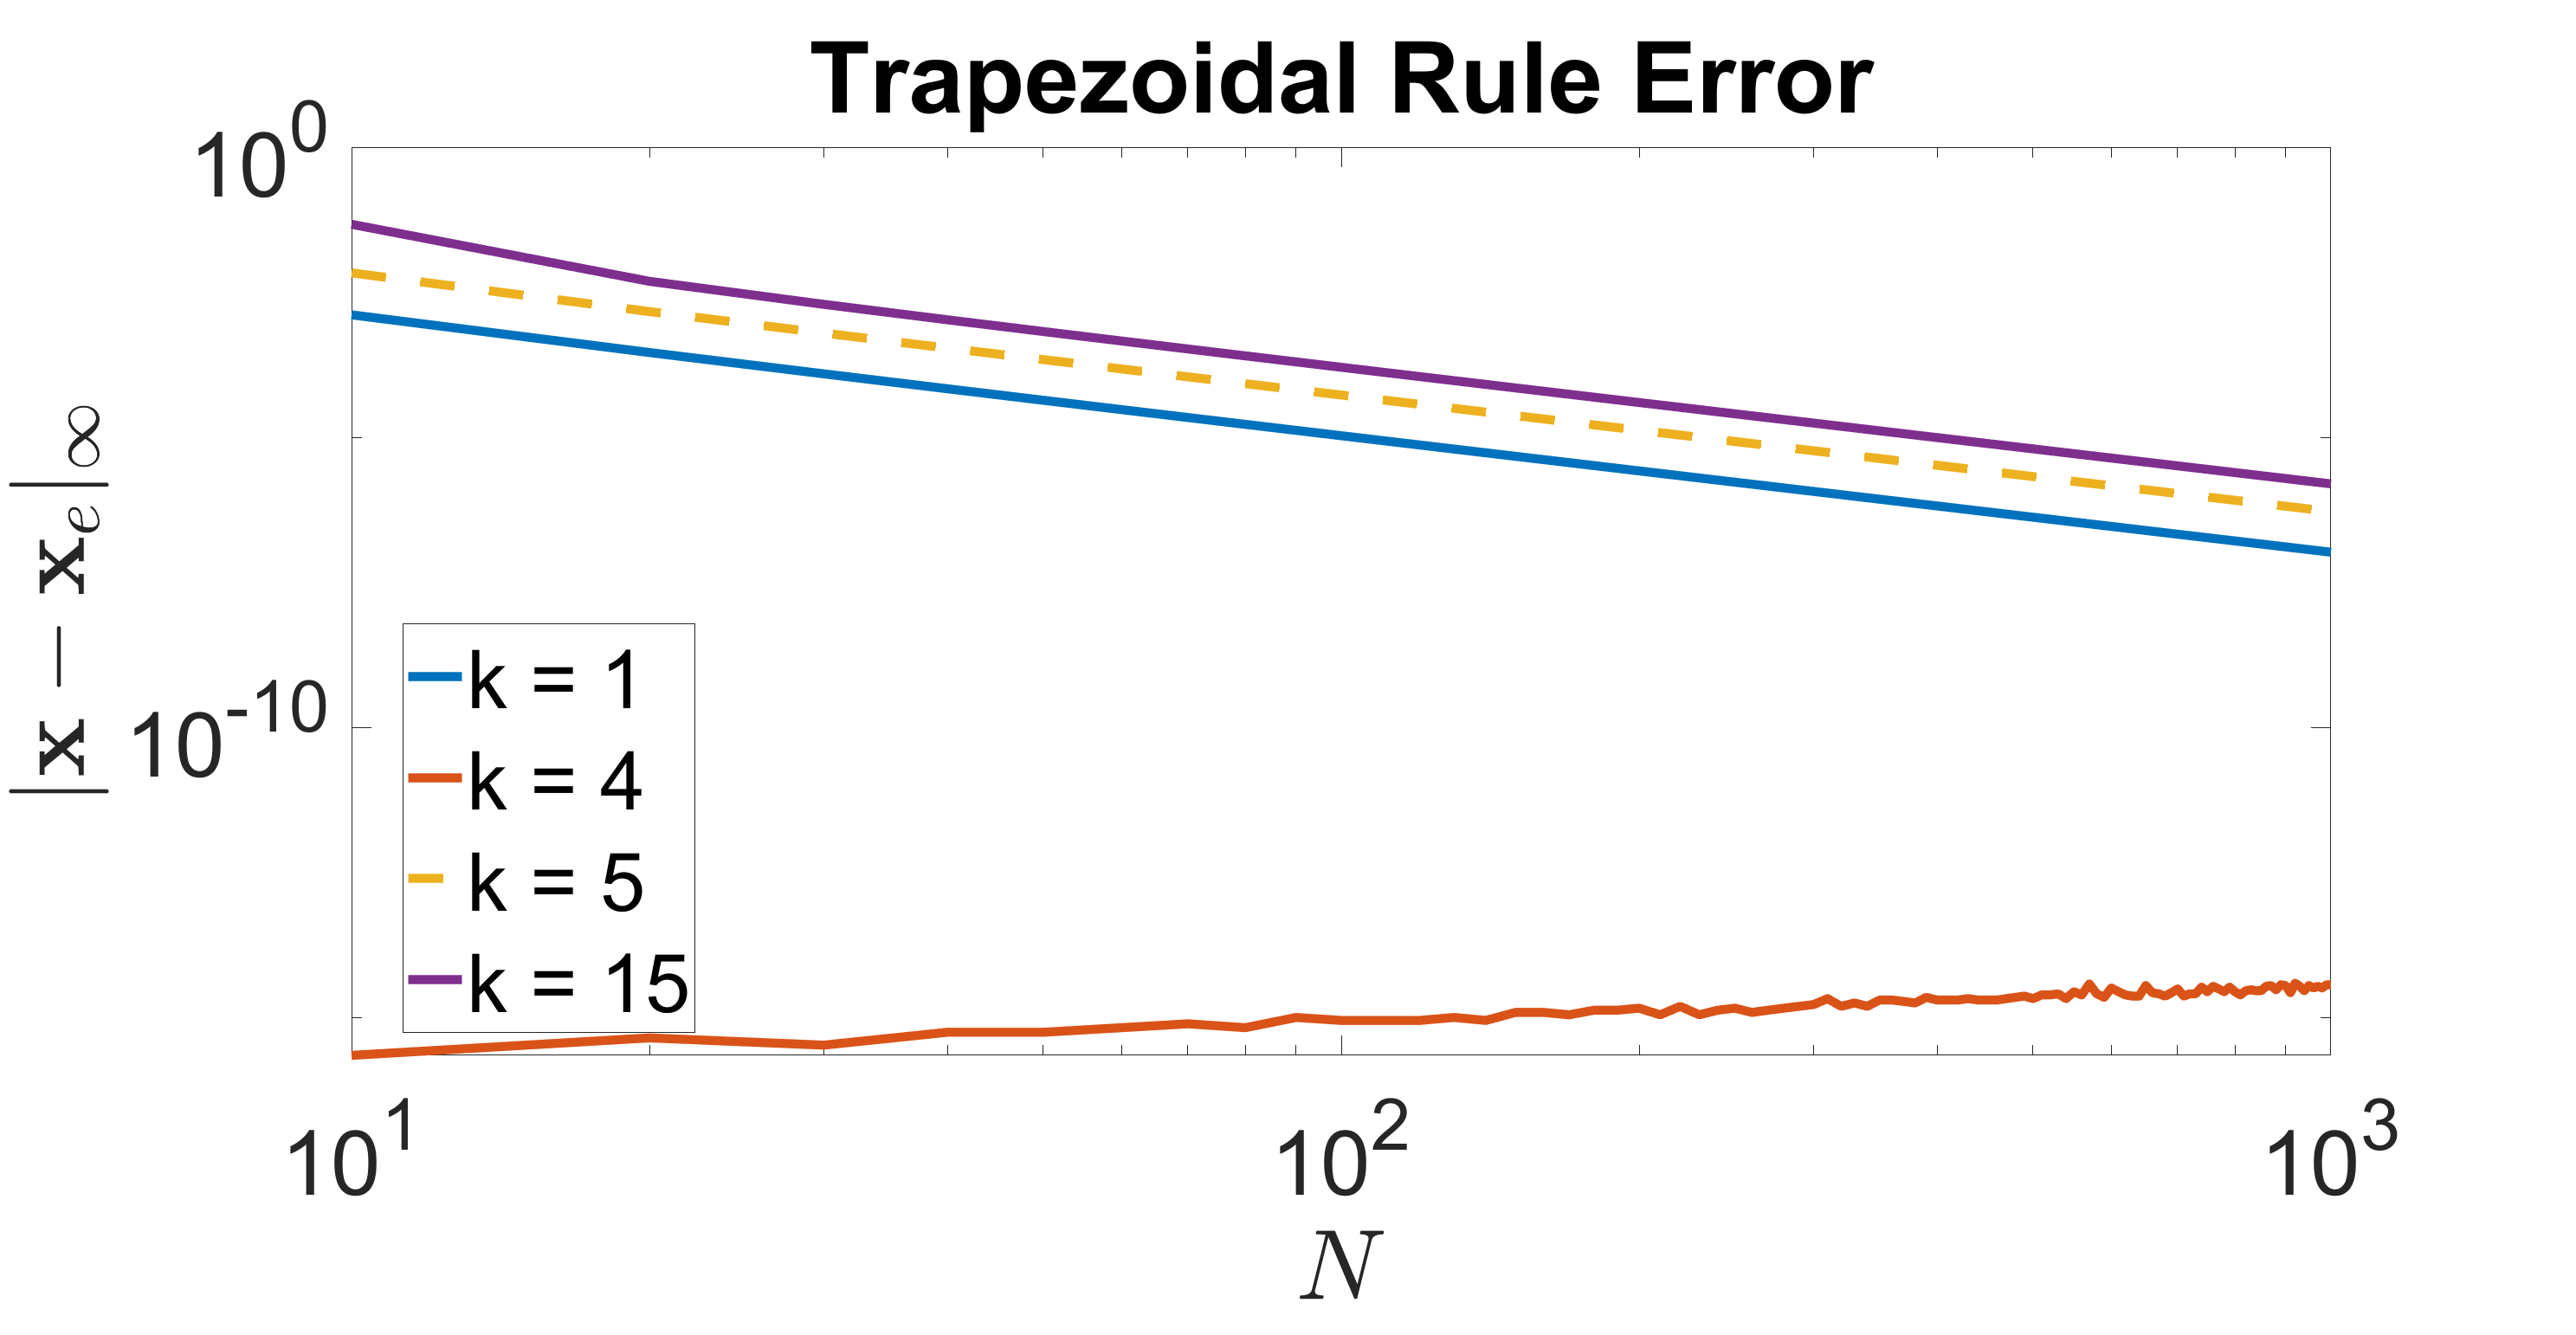
\includegraphics[width=4.5in]{trap_error.png}
    \caption{Maximum error for the trapezoidal rule decay according to some power law. Errors scale uniformly for various $k$: the vertical shift in this plot indicates a proportional decay in error. For $k=4$ and all other even integers, we obtain machine precision error for small $N$. }
    \label{trap_error}
\end{figure}

For $k=4$ and all other even integers, we obtain machine precision error for small $N$. This is due to the symmetric nature of the solution $\cos (ks)$ on the interval $0<s<\pi/2$ when $k$ is even. This symmetry leads to cancellation which gives the correct result. In general this does not occur!

Though we can (using the \texttt{Matlab Turbo-Encabulator}) compute the solution to $10^{-6}$ with the trapezoidal rule, we can easily approximate what necessary resolution is via extrapolation. This is justified in that we know the error scales according to some power law. Performing linear regression on the $\log-\log$ data yields
\vspace{0.15cm}

\texttt{\colorbox{yellow}{\$  For k = 1, error<1e-6 at N = 324}}
\vspace{0.15cm}

\texttt{\$  for k = 1, slope = -2.0202, intercept = -0.92529}
\vspace{0.15cm}

\texttt{\colorbox{yellow}{\$  For k = 4, error<1e-6 at N = 4}}
\vspace{0.15cm}

\texttt{\$  for k = 4, slope = 0.59596, intercept = -16.2534}
\vspace{0.15cm}

\texttt{\$  For k = 5, error<1e-6 at N = 730}
\vspace{0.15cm}

\texttt{\$  for k = 5, slope = -2.0231, intercept = -0.21669}
\vspace{0.15cm}

\texttt{\$  for k = 15, slope = -2.0649, intercept = 0.37311}
\vspace{0.15cm}

\texttt{\colorbox{yellow}{\$  For k = 5, error<1e-6 at N = 1255,}}
\vspace{0.15cm}

thereby confirming our theoretical prediction that the error scales like $N^{-2}$. We also obtain convergence rates from these intercept values. In the log-log plot, translations are synonymous with proportional scaling. In figure \ref{trap_error} we see that the errors behave identically, ignoring a vertical translation. \colorbox{yellow}{The intercepts are the exponents (base 10) of the convergence rates.}

\subsection*{Gauss-Legendre Quadrature}

We give the corresponding errors for Gauss-Legendre quadrature in Figure \ref{gl_error}. We can think of increasing resolution as appending higher order polynomials to our truncated basis. In this way, low order polynomials fail to capture the high frequency modes associated with large $k$. This is illustrated in the figure, where we see the $k = 1$ curve departing from error of order unity early on at small resolutions. The error criterion ($< 10^{-6}$) is satisfied at \colorbox{yellow}{$N = 4$ for $k=1$, $N = 9$ for $k = 4$, and $N = 19$ for $k = 15$}. For the $k = 4$ curve we see a similar departure near the center of the figure. The $k = 15$ curve only departs from unity near the end of the shown resolutions. This behavior is distinctly different from the trapezoidal rule where the approximation appears to get better in a consistent fashion.

\begin{figure}[H]
    \centering
    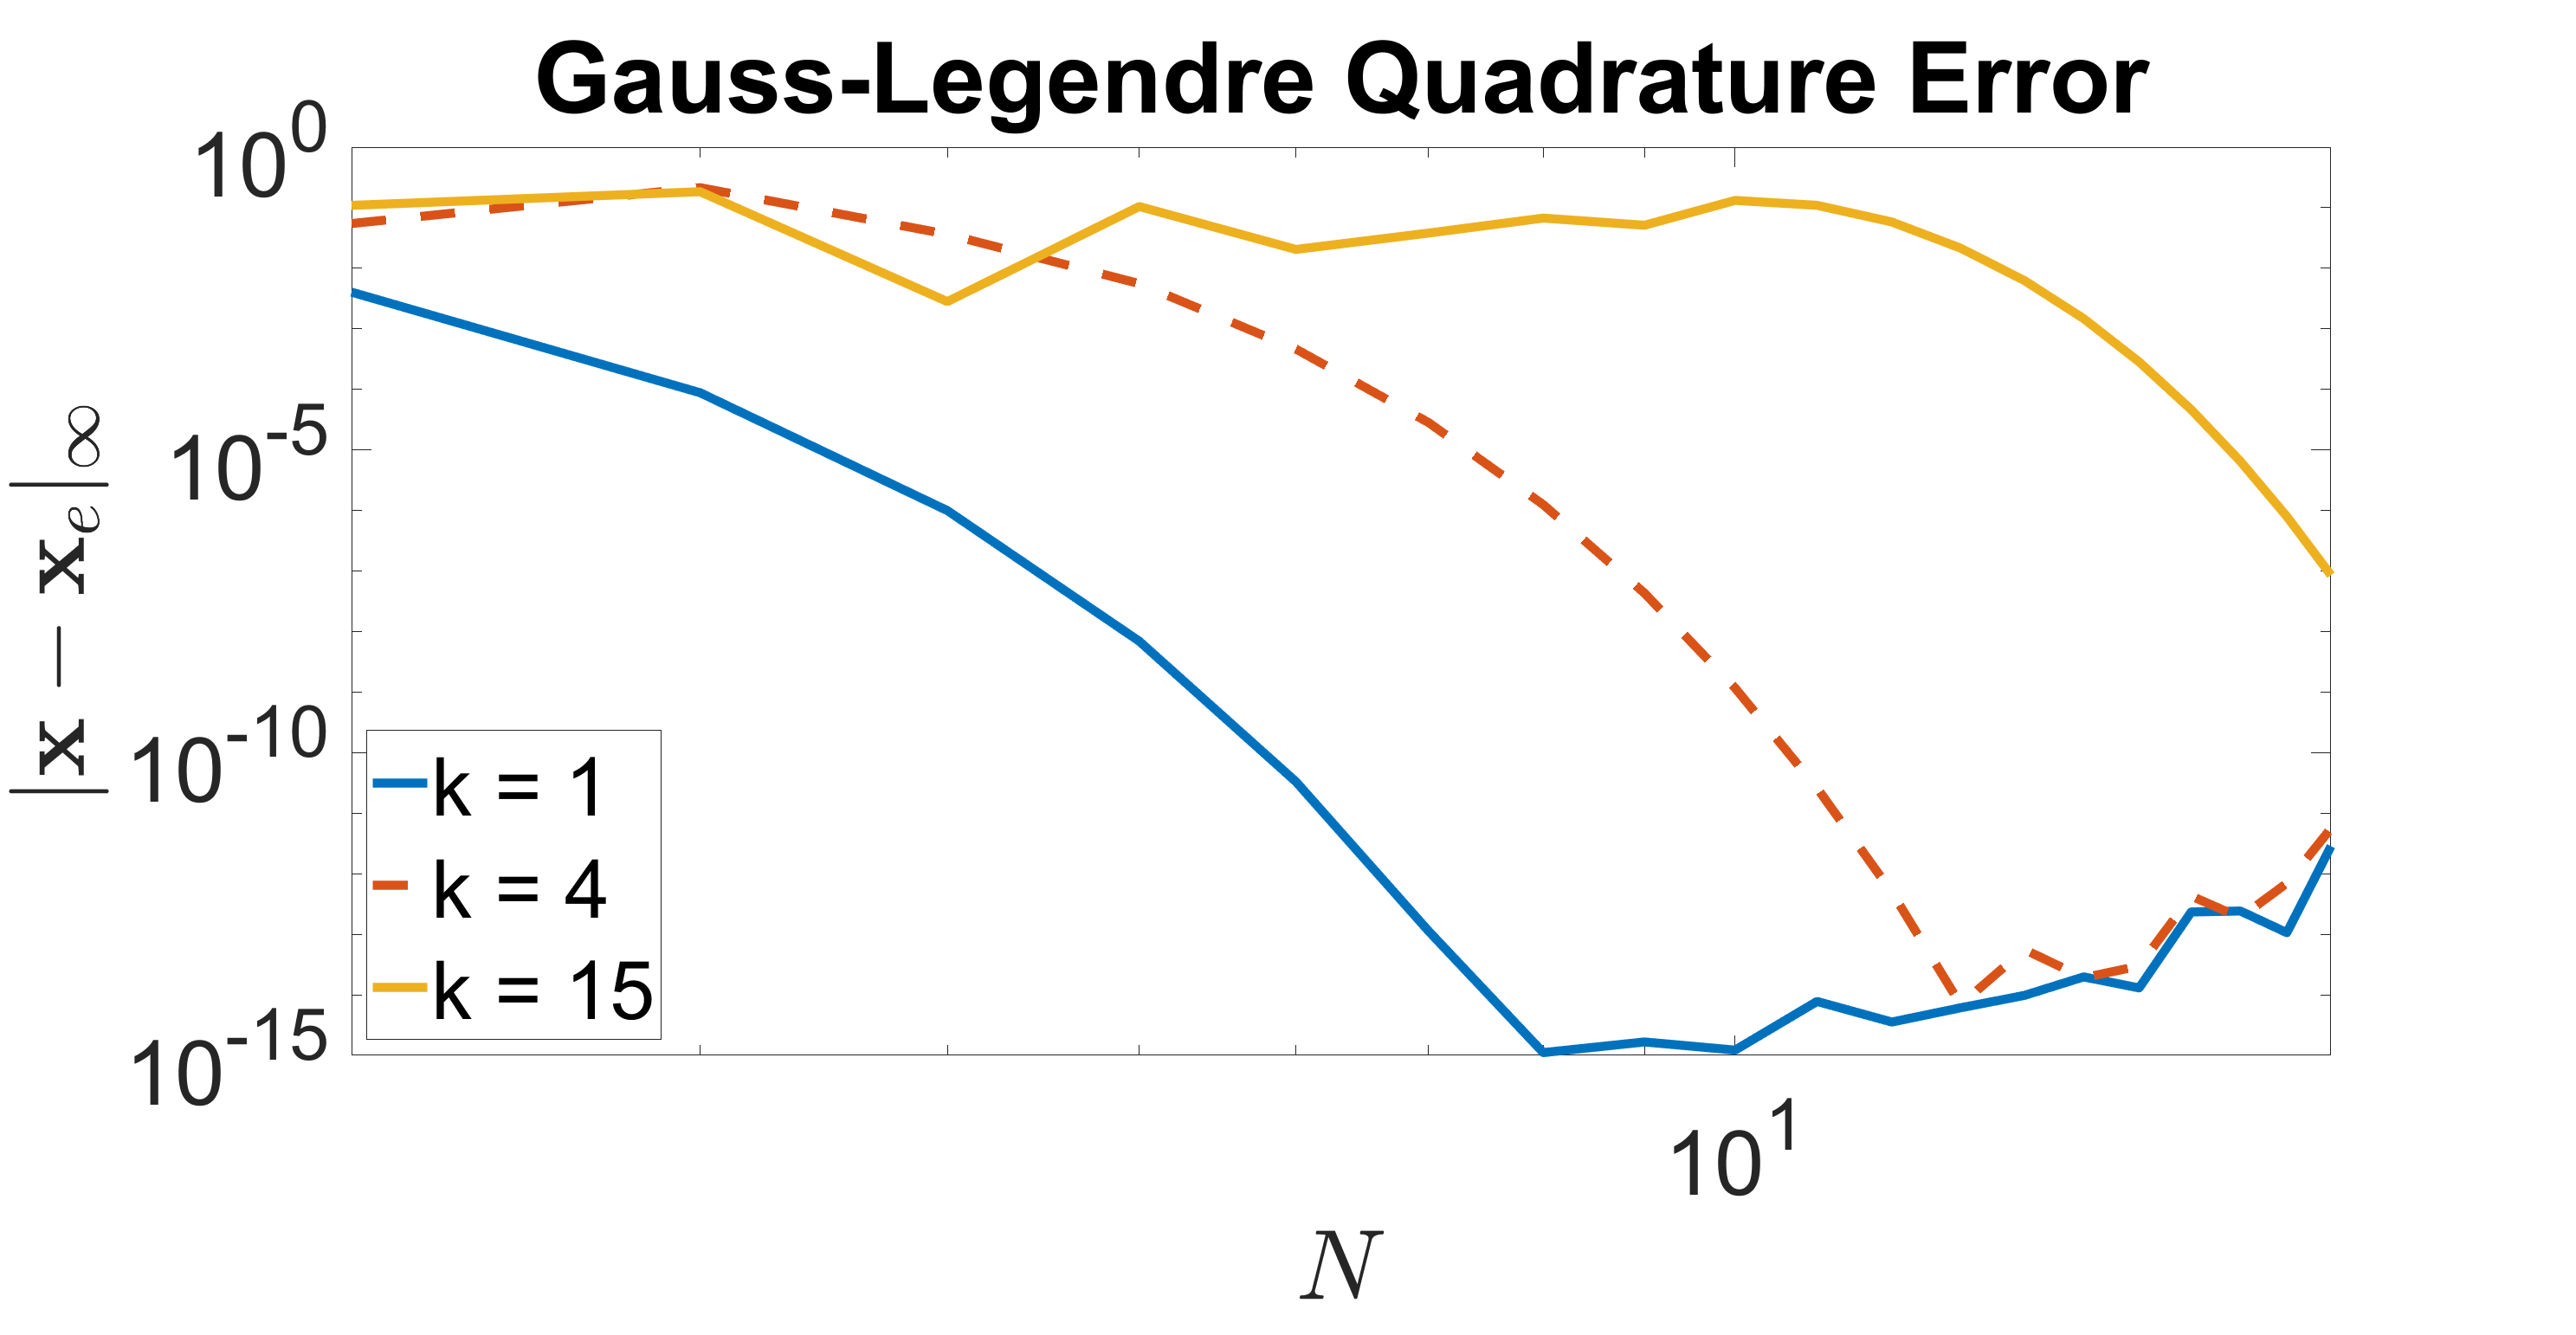
\includegraphics[width=5in]{gl_error.png}
    \caption{Maximum error for Gauss-Legendre quadrature do not decay uniformly according to some power law. In contrast with the trapezoidal rule, the error varies dramatically among different $k$ values at large resolution $N$. Here we satisfy the error $<10^{-6}$ requirement at $N = 4$ for $k = 1$.}
    \label{gl_error}
\end{figure}

Convergence for $k = 15$ is expensive. This is due to the fact that it is a high-frequency function. We can relieve this by making a change of variables $t \to kt$, thereby allowing us to resolve the fast-spatial mode with low resolution.

\section*{Convergence Verification}
Suppose we did not know, a priori, the exact solution. Then the methods outlined above would be useful! We need to be prepared for this in the future.

\subsection*{Gauss-Legendre Quadrature}
 In the case of Gauss-Legendre, due to annihilation, we can employ Taylor's theorem. Recall that smooth/well-behaved functions can be approximated via Taylor series will the error bound being proportional to the supremum of the next highest-order derivative. This ties into the more general and somewhat elusive concept: in order to place restrictions on the error to make statements about convergence, we need to have some sort of information about the length-scale of the function. Otherwise the concept of discretization is meaningless. In this case, from the text, we can claim that the error $|Ef|$ of the quadrature of a function $f$ on an interval $(a, b)$ is approximattely bounded by 
\begin{align*}
    |Ef| &\lesssim 4 \sup |f^{(2N)}| \sqrt{\frac{N}{\pi}} \Big( \frac{e}{N} \Big)^{2N}
\end{align*}
where we know in this case $\sup |f^{(2N)}| = 2kN$. This explains why the high-frequency mode is so difficult to approximate! In this case $8k/\sqrt{pi}$ serves as a convergence rate as it is the proportionality constant between the error approximation and some function of resolution.

\subsection*{Trapezoid Rule}
For the Trapezoid rule we can examine the error in a controlled scenario. For example, letting $k = 1$ we have that the quadrature integrand $\cos s$ on $(0, \pi/2)$ is strictly concave down. It follows that the trapezoid rule with \textit{always} underestimate the region of integration. Thus as we increase $N$ the integral estimate grows monotonically. It follows from the \textit{Monotone Convergence Theorem} that the desired sum is the supremum of this sum of all estimates. This, combined with the fact that we know that the error must scale like $N^{-2}$ allows us to estimate the error. Recall that the approximation is accurate to machine precision for even $k$ due to symmetry, so we will curtail our discussion to odd $k$. If we had some information about the integrand (important), we could bound the error
\begin{align*}
    |Ef| &\leq \frac{\sup |f''(s)|}{12N^2}(b - a)^3
\end{align*}
as before. Here $\sup |f''(s)| = 2k$. Thus our convergence factor is given by $\frac{k\pi^3}{24}$.

\end{document}
